% "Aufbau.tex" --- Kapitel 3 f�r das Template "Auswertung.tex"
%
% Wolfgang Sch�pf, Januar 2013
% letzte �nderung: 

\chapter{Messprotokoll: Versuchsaufbau, Messmethoden und Durchf�hrung}
\label{chap:aufbau}
%
\section{Einf�gen von Abbildungen}
\label{sec:abbildung}
%
\subsection{Die \texttt{figure}--Umgebung}
\label{subsec:figure}

% Hier wird nun die erste Abbildung erzeugt:
%
\begin{figure}[b]
\begin{center}
  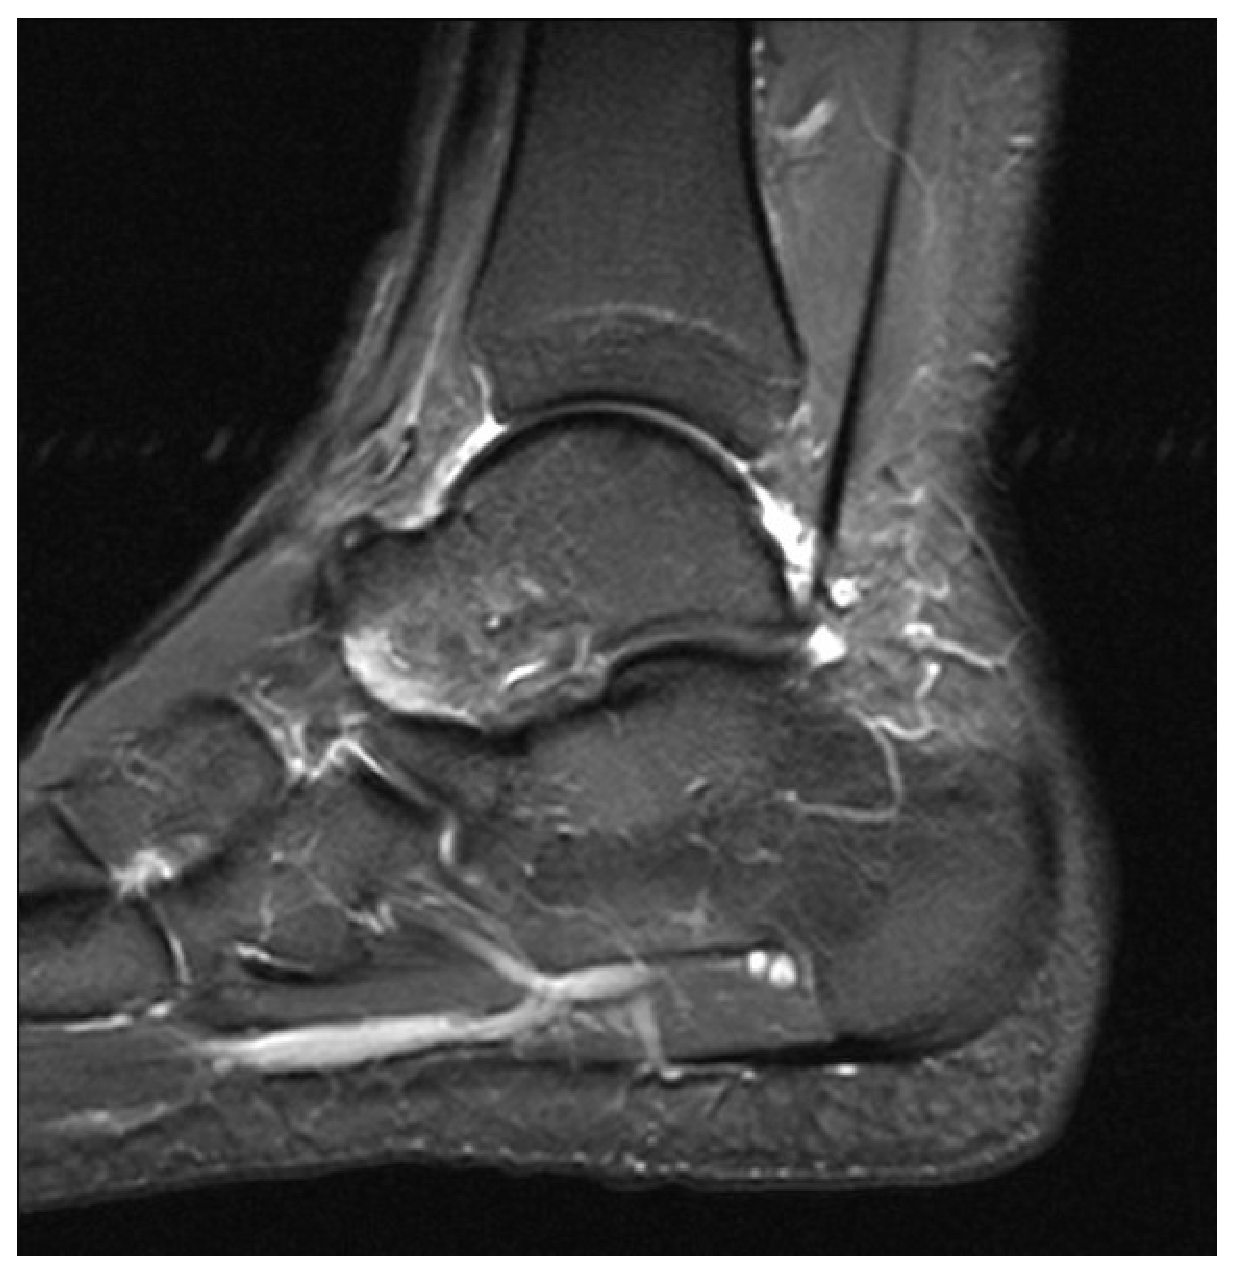
\includegraphics[width = 0.5 \textwidth]{./bilder/Fuss_Kernspin}
  \caption{\label{fig:kernspin} Kernspintomogramm eines menschlichen Fu�es.}
\end{center}
\end{figure}

Das Einf�gen von Abbildungen erfolgt am Einfachsten mit Hilfe der \verb+figure+--Umge\-bung 
und ist exemplarisch in Abb.~\ref{fig:kernspin} gezeigt.%
%
\footnote{Abbildung~\ref{fig:kernspin} wurde aus \citet{Kramer2010} entnommen.} 
%
Diese Umgebung, wie auch die in Abschnitt~\ref{sec:tabelle} besprochene \verb+table+--Umgebung, 
ist beweglich, d.\,h.\ \LaTeX\ entscheidet nach gewissen Kriterien, wohin die Abbildung platziert 
wird. Zus�tzlich k�nnen beim �ffnen der Umgebung ein oder mehrere Positionierungsparameter 
angegeben werden, wobei die Sinnvollsten `h' f�r 'here', `t' f�r 'top' und `b' f�r 'bottom' sind:
\verb+\begin{figure}[htb]+. Die Reihenfolge dieser Parameter priorisiert die Wahl der Platzierung.

\begin{sloppypar}
%
Innerhalb der Umgebung kann eine Bildunterschrift mit Hilfe des Befehls 
\verb+\caption{... text ...}+ erzeugt werden. Au�erdem sollte jede Abbildung mit einem Label
versehen werden, um leicht darauf Bezug nehmen zu k�nnen, wie dies im vorhergehenden Absatz 
geschehen ist. Ganz allgemein sollten Bilder und Tabellen nie einfach so im Dokument erscheinen,
sondern \textbf{immer} im Text auch referenziert werden.
%
\end{sloppypar}

\subsection{Einbinden des Bildes}
\label{subsec:bild}
%
Das einzubindende Bild sollte m�glichst als eps--Datei vorliegen bzw.\ in eine solche 
konvertiert werden. Das Bild kann sich im aktuellen Arbeitsverzeichnis oder in dem durch
\verb+\graphicspath{{./bilder/}}+ festgelegten Verzeichnis befinden, es kann beim Einbinden aber 
auch der Pfad direkt angegeben werden. Das Einbinden selbst geschieht durch den Befehl
%
\begin{verbatim}
   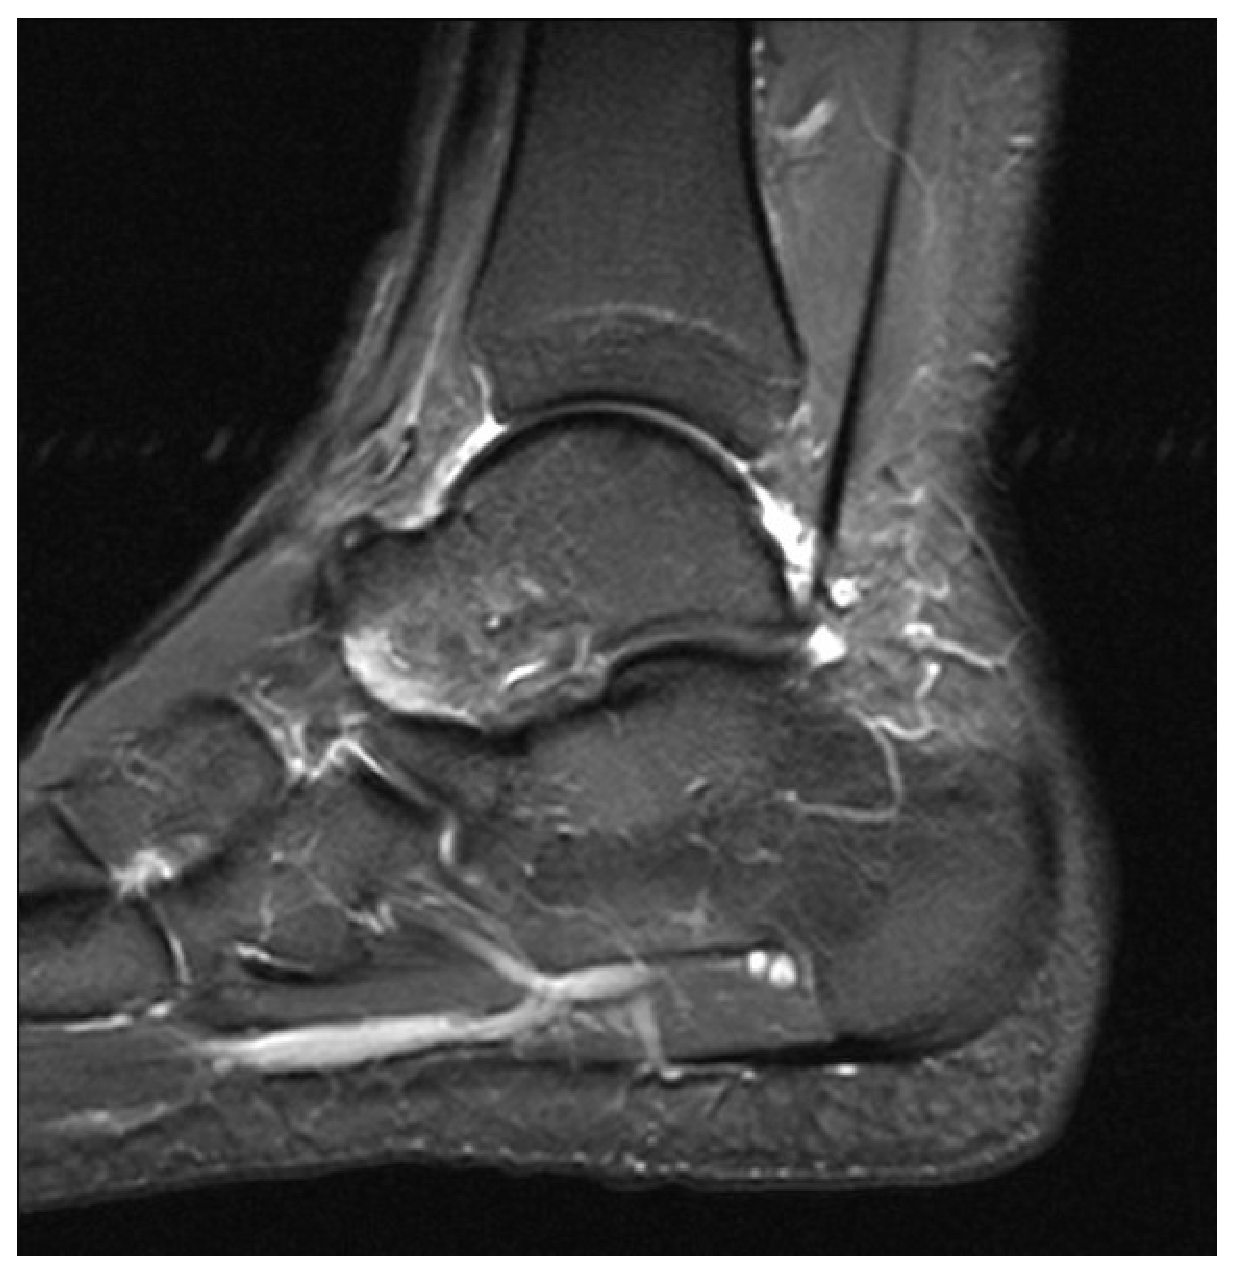
\includegraphics[width = 0.5\textwidth]{./bilder/Fuss_Kernspin}
\end{verbatim}
%
Hier ist es sinnvoll, als Parameter entweder die Breite (\verb+width+) oder die H�he 
(\verb+height+) anzugeben, und zwar m�glichst in Einheiten der Textbreite (\verb+\textwidth+)
bzw.\ der Texth�he (\verb+\textheight+). Beim Einbinden von Abbildungen k�nnen auch 
kompliziertere Konstruktionen verwendet werden, wie in Abb.~\ref{fig:MM} gezeigt.

% Hier wird eine etwas kompliziertere Abbildung erzeugt:
%
\begin{figure}[h]
    \begin{minipage}{0.2\textwidth}
        \centerline{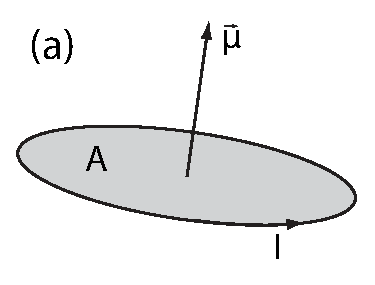
\includegraphics[width = \textwidth]{bilder/MM_MagnetischesMoment}}
    \end{minipage} 
    \hfill
    \raisebox{0.2cm}{
        \begin{minipage}{0.55\textwidth}		
        \caption{\label{fig:MM} \newline
                 Magnetisches (Dipol-)Moment $\vec{\mu}$ \protect\\ 
                 (a) einer kreisf\"ormigen Leiterschleife und \protect\\ 
                 (b) eines Permanentmagneten mit Nord- (N) und S\"udpol (S).%
                 \protect\footnote{Dieses Bild wurde aus \citet{Kramer2010} entnommen.}
                 }
        \end{minipage} 
        }
    \hfill
    \begin{minipage}{0.19\textwidth}
        \centerline{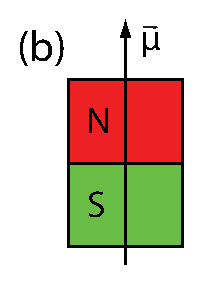
\includegraphics[height = \textwidth]{bilder/MM_Permanentmagnet}}
    \end{minipage} %}
\end{figure}

\section{Einf�gen von Tabellen}
\label{sec:tabelle}
%
\subsection{Die \texttt{table}--Umgebung}
\label{subsec:table}
%
Die \verb+table+--Umgebung ist sehr �hnlich zur \verb+figure+--Umgebung und eignet sich zum 
Einf�gen von Tabellen in den Text. Sie ist, wie schon erw�hnt, ebenfalls beweglich und l�sst die
gleichen Positionierungsparameter zu. Innerhalb der Umgebung kann eine Tabellenbeschriftung
erzeugt werden und auch Tabellen sollten immer ein Label erhalten. Ein sehr einfaches Beispiel
stellt Tab.~\ref{tab:mears} dar.

\subsection{Erstellen von Tabellen}
\label{subsec:tabular}
%
Eine Tabelle wird am Zweckm��igsten mit Hilfe der \verb+tabular+--Umgebung erstellt, wie dies
auch bei Tab.~\ref{tab:mears} geschah. Die Formatierung der Spalten wird beim �ffnen der Umgebung
bestimmt, z.\,B.\ \verb+\begin{tabular}{c||c|l|l|c|r}+. Diese Tabelle besteht aus 6 Spalten, wobei
der Inhalt der Spalten 1, 2 und 5 horizontal zentriert ist (c), der Inhalt der Spalten 3 und 4
wird linksb�ndig dargestellt (l), w�hrend Spalte 6 rechtsb�ndig erscheint (r). \verb+|+ erzeugt
einen vertikalen Strich zwischen zwei Spalten, \verb+||+ erzeugt zwei dicht benachbarte Striche.
Die Eintr�ge in den einzelnen Spalten werden durch \verb+&+ voneinander getrennt, \verb+\\+
beendet eine Zeile. Ein horizontaler Strich wird durch \verb+\hline+ nach dem Zeilenende eingef�gt.

% eine erste einfache Tabelle
%
\begin{table}[t]
\raisebox{0.2cm}{ 
    \begin{minipage}{0.3\textwidth}			
    \caption{\label{tab:mears} \newline
              Literaturwerte f\"ur B(T) \protect\\ \citep{Mears1969}}
    \end{minipage} 
}
\hfill
\begin{minipage}{0.57\textwidth}
    \begin{tabular}{c||c|c|c|c|c}
    $T$ / $^{\circ}$C                      & 20   & 30   & 40   & 50   & 60 \\[.5ex]
    \hline  & & & & & \\[-2.5ex]
    $B$ / $\frac{\text{cm}^3}{\text{mol}}$ & -294 & -275 & -257 & -235 & -223
    \end{tabular}
\end{minipage}
\end{table}

Eine etwas kompliziertere Tabelle ist aus \citet{Khazimullin2011} entnommen und in Tab.~\ref{tab:gamma_1}
gezeigt. Der Aufbau wird durch Lesen des Quelltextes klarer. Die dabei auftretenden \verb+$+--Zeichen 
f�r den mathematischen Modus werden im n�chsten Abschnitt erl�utert. Der Befehl 
\verb+\multicolumn{3}{c}{Homopolymer}+ fasst mehrere Spalten zu einer zusammen. In diesem Fall werden 
3 Spalten zu einer, in der das Wort ``Homopolymer'' zentiert erscheint, kombiniert. �hnlich wurde die
�berschrift ``Block copolymer'' erzeugt.

\begin{table}[h]
\begin{center}
    \begin{tabular} {@{\extracolsep{1ex}}cccc|ccc}
        \multicolumn{4}{c|}{Block copolymer} & \multicolumn{3}{c}{Homopolymer} \\
        c (\%) & $\gamma_1$ (Pa$\cdot$s) & $2 \sigma$ (Pa$\cdot$s) & & c (\%) & $\gamma_1$ (Pa$\cdot$s) & $2 \sigma$ (Pa$\cdot$s) \\
        \hline
        0.2 & 0.081 & 0.011 & & 0.5 & 0.114 & 0.025 \\
        0.5 & 0.10  & 0.02  & & 1.0 & 0.17  & 0.05 \\
        0.8 & 0.16  & 0.03  & & 1.5 & 0.37  & 0.09 \\
        1.1 & 0.23  & 0.07  & & 2.0 & 0.49  & 0.07 \\
        1.3 & 0.51  & 0.15  & & 2.5 & 0.81  & 0.23 \\
        1.5 & 0.73  & 0.15  & & \\
        1.8 & 2.4   & 1.3   & & \\
        2.1 & 11    & 3.8   & & \\
        2.3 & 47    & 38    & & \\
    \end{tabular}
\caption{\label{tab:gamma_1} Measured rotational viscosity $\gamma_1$ with the corresponding 
         standard deviation $2 \sigma$ for all polymer samples. For pure 5CB, we found 
         $\gamma_1 = 0.078\,$Pa$\cdot$s with $2 \sigma = 0.010\,$Pa$\cdot$s.}
\end{center}
\end{table}

